\documentclass{article}

\usepackage{graphicx}
\usepackage{tikz}
\usepackage{tikzsymbols}
\usetikzlibrary{calc,patterns,shapes.geometric}
\pagestyle{empty}
\usepackage[margin=0pt]{geometry}
\geometry{papersize={14in,12in}}

\def\centerarc[#1](#2)(#3:#4:#5){\draw[#1] ($(#2)+({#5*cos(#3)},{#5*sin(#3)})$) arc (#3:#4:#5);}

\begin{document}
	\begin{figure}
		\centering
		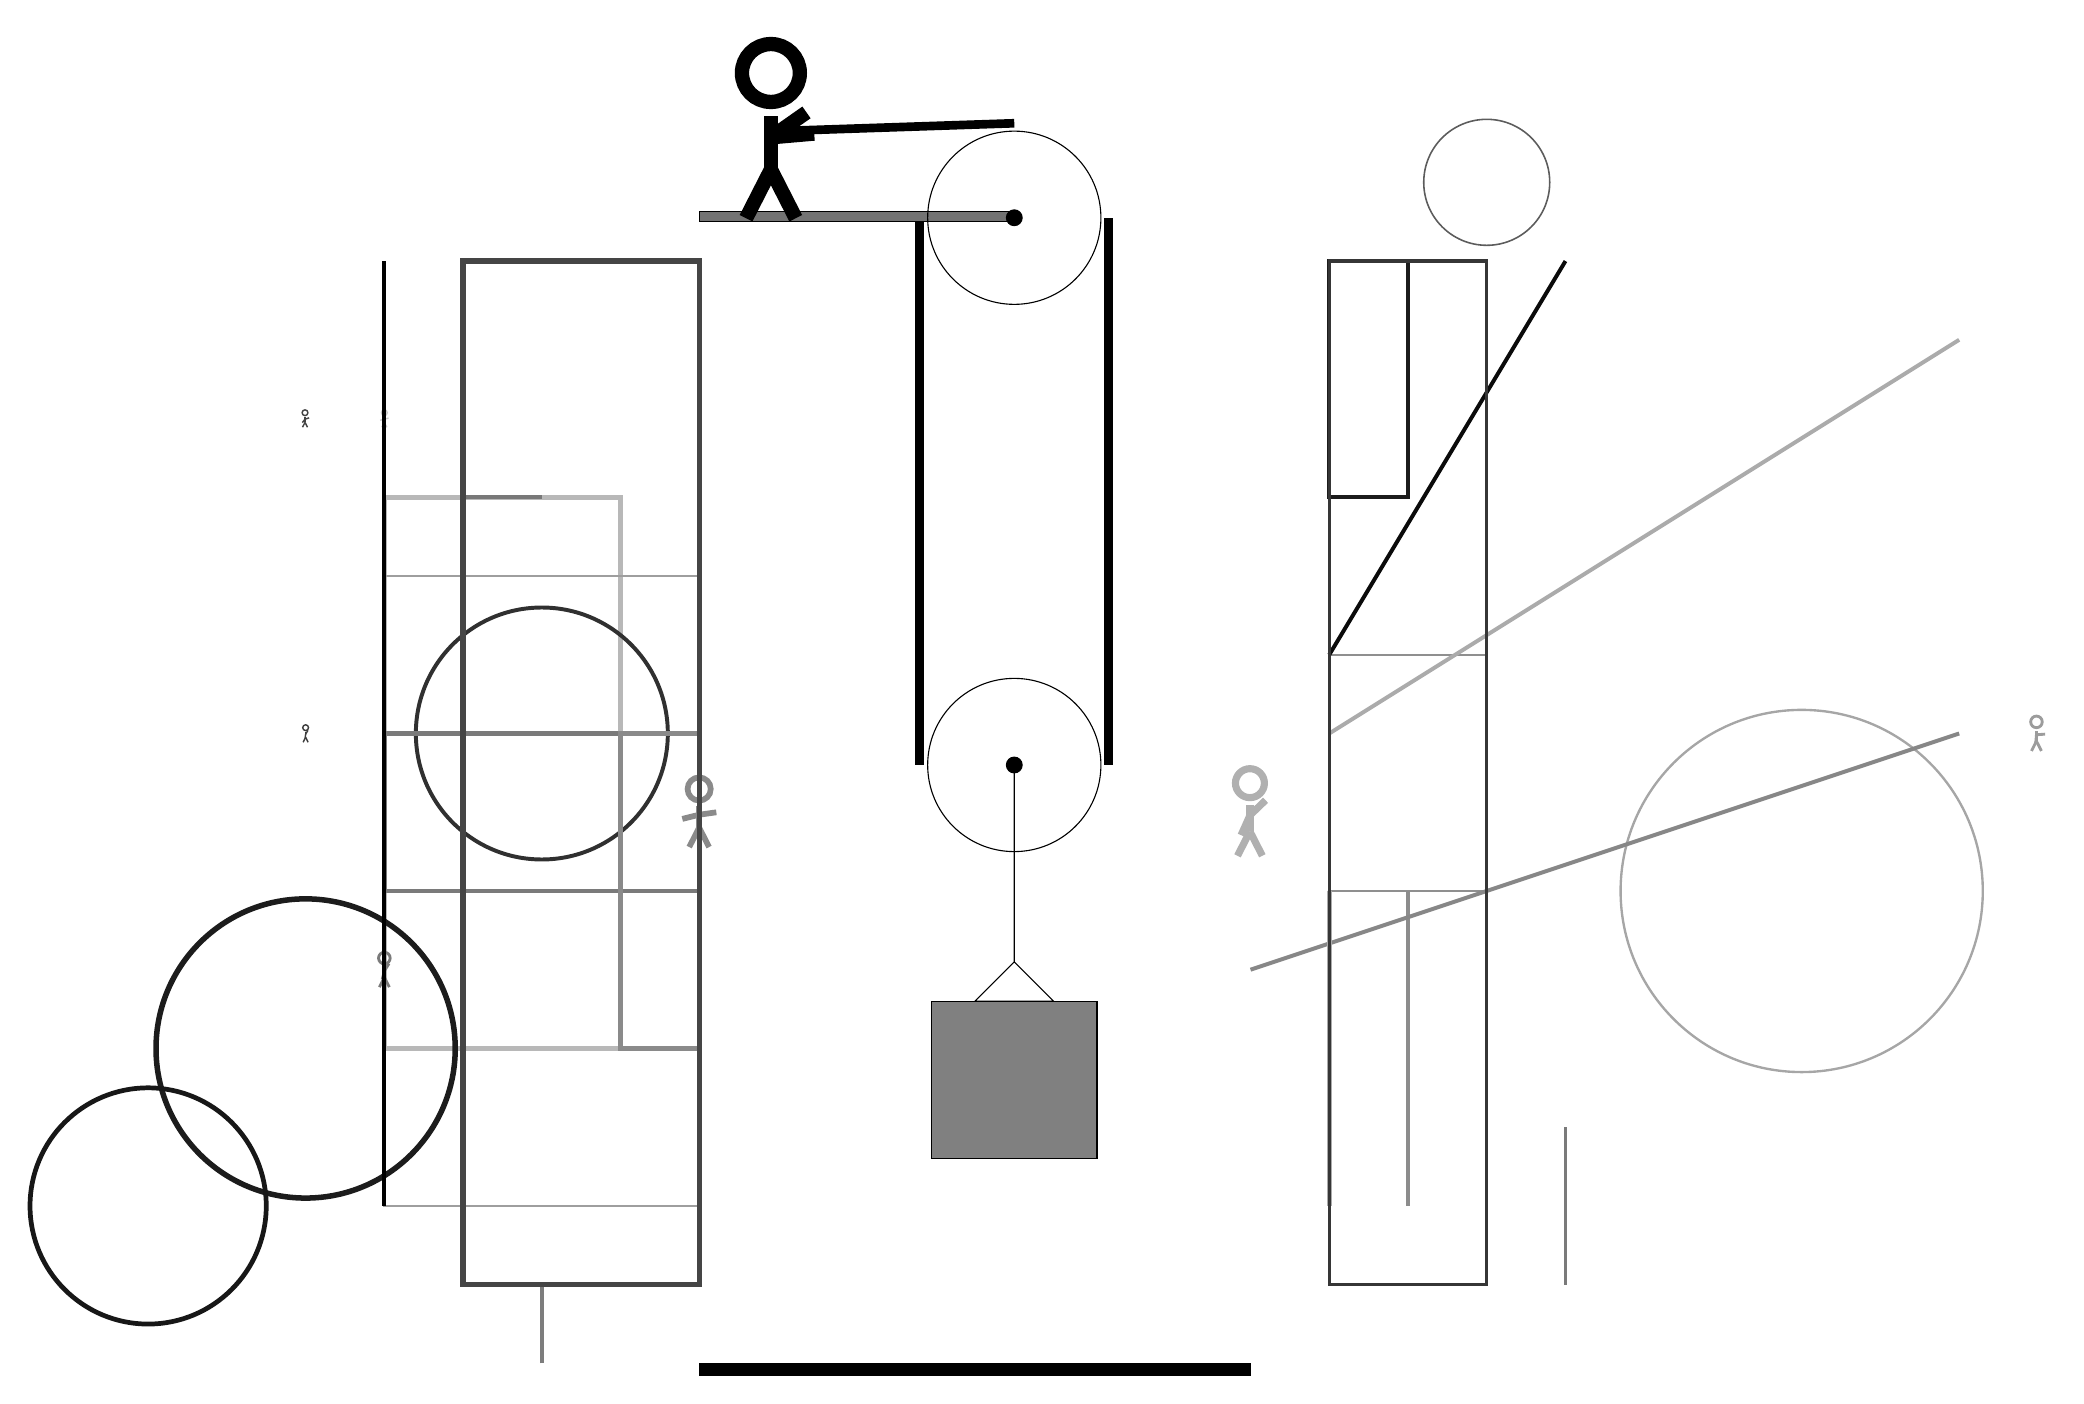
\begin{tikzpicture}
			%%%%% START %%%%%
			
			\draw[fill=black!55] (-2, 11.5) rectangle (2, 11.625);
			
			\draw (2, 4.6) circle (1.1);
			\draw[fill=black] (2, 4.6) circle (0.1);
			
			\draw (2, 11.55) circle (1.1);
			\draw[fill=black] (2, 11.55) circle (0.1);
			
			\draw (2, 4.6) -- (2, 2.1) -- (1.5, 1.6) -- (2.5, 1.6) -- (2, 2.1);
			\draw[fill=black!50] (0.95, 1.6) rectangle (3.05, -0.4);
			
			\draw[line width=1.1mm] (0.8, 11.5) -- (0.8, 4.6);
			\centerarc[line width=1.1mm](2, 4.6)(180:360:1.2000000000000002);
			\draw[line width=1.1mm](3.2, 4.6) -- (3.2, 11.55);
			\centerarc[line width=1.1mm](2, 11.55)(0:90:1.2000000000000002);
			\draw[line width=1.1mm](2, 12.75) -- (-1, 12.65);
			
			\node[line width=0.6mm, color=black!39] at (15, 5) {\Strichmaxerl[2][85][4]};
			
			\draw [line width=0.2mm, color=black!64](8, 12) circle (0.8);
			\node[line width=0.5mm, color=black!21] at (-6, 9) {\Strichmaxerl[1][15][14]};
			\draw[line width=0.5mm, color=black!52](9, -2) -- (9, 0);
			\draw[line width=0.2mm, color=black!44] (6, 3) rectangle (8, 6);
			
			\draw[line width=0.6mm, color=black!28] (-3, 8) rectangle (-6, 1);
			
			\draw[line width=0.3mm, color=black!38] (-2, -1) rectangle (-6, 7);
			\node[line width=0.2mm, color=black!76] at (-7, 5) {\Strichmaxerl[1][84][58]};
			\draw[line width=0.5mm, color=black!53](-5, 8) -- (-4, 8);
			
			\node[line width=0.6mm, color=black!31] at (5, 4) {\Strichmaxerl[5][66][44]};
			
			\draw[line width=0.5mm, color=black!45](7, 3) -- (7, -1);
			\draw [line width=0.5mm, color=black!81](-4, 5) circle (1.6);
			\draw[line width=0.6mm, color=black!52] (-2, 5) rectangle (-6, 3);
			\draw[line width=0.5mm, color=black!51](-4, -3) -- (-4, -2);
			\draw [line width=0.3mm, color=black!35](12, 3) circle (2.3);
			\draw[line width=0.5mm, color=black!47](5, 2) -- (14, 5);
			\draw[line width=0.7mm, color=black!46] (-3, 1) rectangle (-2, 5);
			\draw [line width=0.7mm, color=black!89](-7, 1) circle (1.9);
			\draw[line width=0.5mm, color=black!96](9, 11) -- (6, 6);
			\node[line width=0.6mm, color=black!52] at (-6, 2) {\Strichmaxerl[2][76][58]};
			\draw[line width=0.6mm, color=black!33] (6, -1) rectangle (6, 3);
			\draw[line width=0.5mm, color=black!89] (6, 8) rectangle (7, 11);
			
			\node[line width=0.6mm, color=black!74] at (-7, 9) {\Strichmaxerl[1][52][18]};
			\node[line width=0.2mm, color=black!46] at (-2, 4) {\Strichmaxerl[4][14][8]};
			\draw[line width=0.5mm, color=black!100](-6, -1) -- (-6, 11);
			
			\draw [line width=0.6mm, color=black!91](-9, -1) circle (1.5);
			\draw[line width=0.5mm, color=black!33](6, 5) -- (14, 10);
			\draw[line width=0.4mm, color=black!79] (6, -2) rectangle (8, 11);
			\draw[line width=0.7mm, color=black!73] (-2, -2) rectangle (-5, 11);
			
			
			\node at (-1, 12.65) {\Strichmaxerl[10][-175][35]};
			
			\draw[fill=black] (-2, -3) rectangle (5, -3.15);
			
			%%%%% END %%%%%
		\end{tikzpicture}
	\end{figure}	
\end{document}